\chapter{Introduction} % (fold)
\label{cha:intro}


\begin{abstract}
This chapter places this dissertation in the context of
modern societies and their challenges. Specifically, we
motivate this thesis by the demographic changes in the
global North. In the process, we identify
\acl{tg} as a central problem in robotics, recall existing
approaches and discuss their limitations. Finally, we
present the contributions and the outline of this
dissertation.
\end{abstract}

\newpage


As the countries of the global North are struggling with the
challenges of an aging population, shifting demographics
(\cref{fig:demographic_change}), and a scarcity of
affordable labor for physically demanding tasks, the need
for technological solutions is more pronounced than ever
\cite{ince2015economic,mcgrath2021report,astrov2021economies}.
Technological progress in the
corresponding field of robotics today is disappointing,
especially in an era where the non-embodied counterpart,
i.e. speech recognition \cite{radford2023robust},
text generation \cite{hoffmann2022training},
and computer vision \cite{voulodimos2018deep}, is
touching all of our lives. Specifically, strides in natural
language processing and computer vision have significantly
improved in the recent past and may rather sooner than later
increase our productivity substantially. In contrast, 
embodied systems still lag behind in
sophistication and are still mainly bound to industrial
settings.

\begin{figure}[ht]
  \begin{subfigure}{0.5\textwidth}
    \centering
    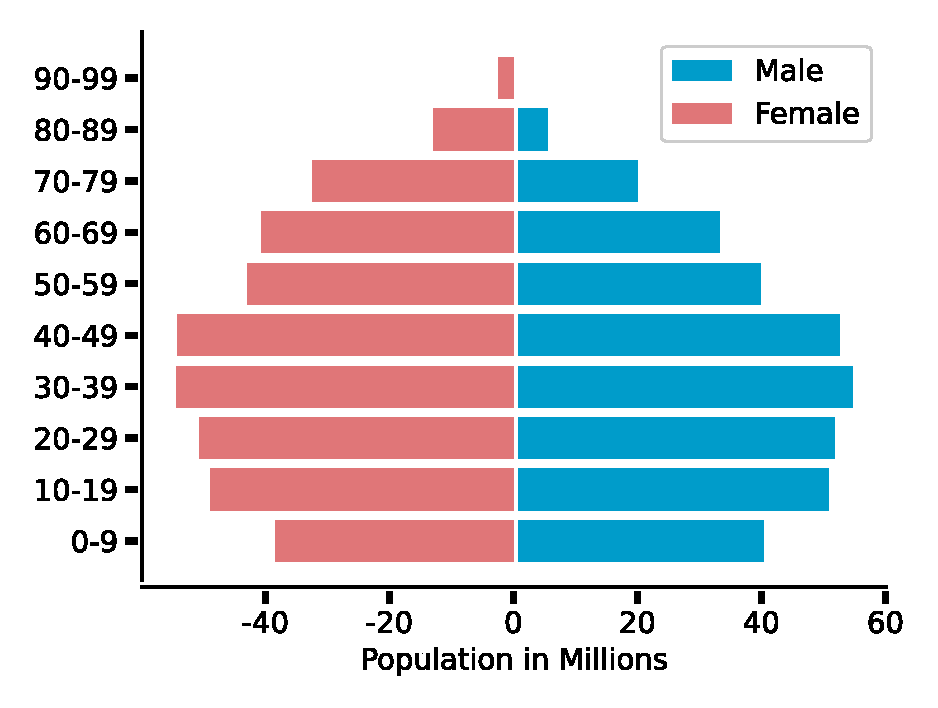
\includegraphics[width=0.9\textwidth]{src/introduction/img/population_2000.eps}
  \end{subfigure}%
  \begin{subfigure}{0.5\textwidth}
    \centering
    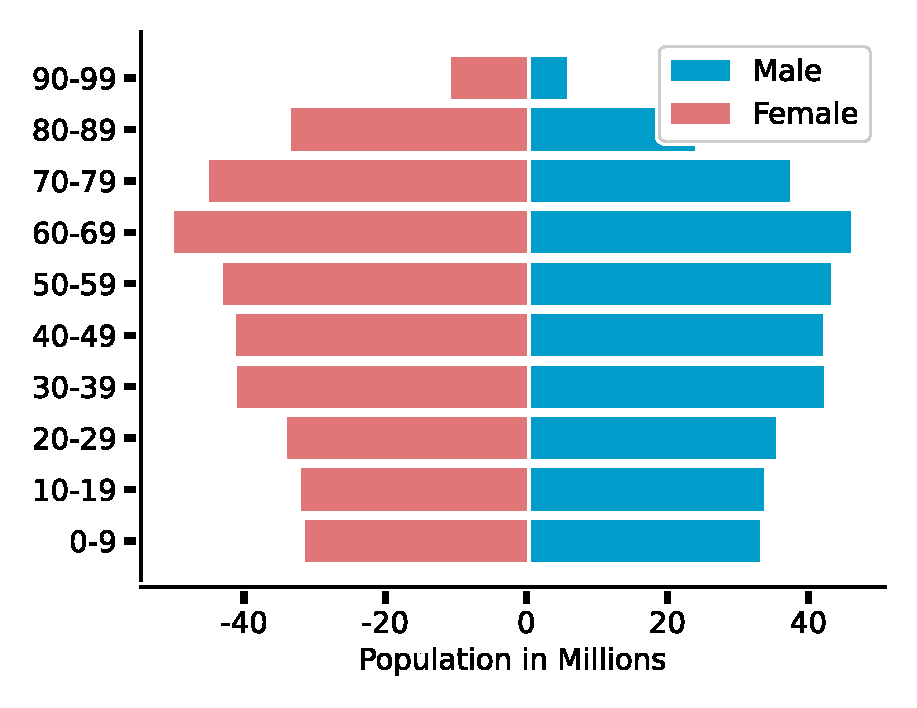
\includegraphics[width=0.9\textwidth]{src/introduction/img/population_2050.eps}
  \end{subfigure}
  \caption
  []
  {
    Population portions by age in 2000 (left) and predictions for
    2050 (right) in Europe \footnotemark. The aging society leads to labor shortage
    which may be counterbalanced with increase in
    automation.
  }
  \label{fig:demographic_change}
\end{figure}

\footnotetext{
    United Nations, Department of
    Economic and Social Affairs, Population Division (2022)
}
% Safety
Industrial robots, see \cref{fig:industrial_robot}
are highly capable in certain tasks, but
these systems are often unable to adapt to changes in
real-time and lack the nuanced understanding and safety required for
dynamic, human-shared environments. Collaborative robots
promote safety through a lightweight
hardware design and a broader set of sensors, see
\cref{fig:collaborative_robot}. These
robots are designed to exist safely alongside their human
counterparts using different low-level control approaches.
%
\begin{figure}[t]
  \centering
  \begin{subfigure}{0.5\textwidth}
    \centering
    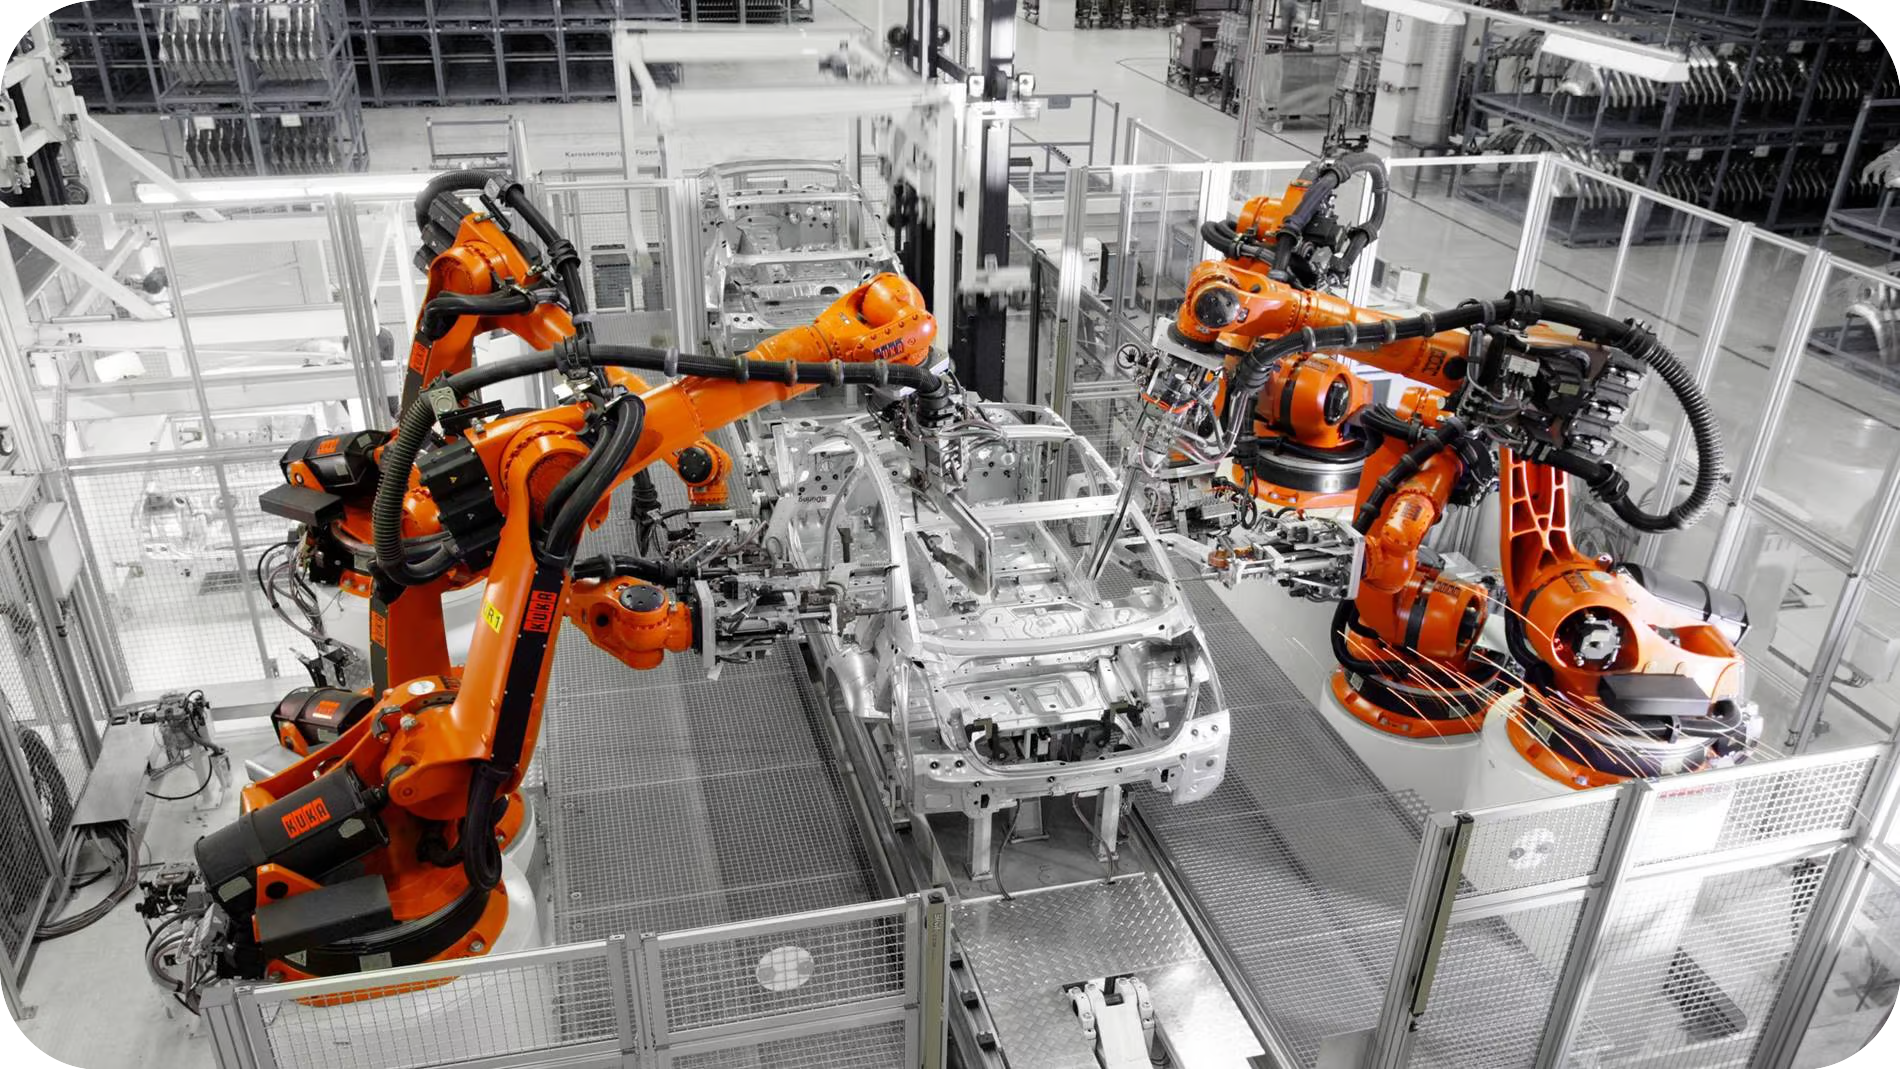
\includegraphics[width=0.9\textwidth]{src/introduction/img/industrial_robot.png}
    \caption{Industrial robot}
    \label{fig:industrial_robot}
  \end{subfigure}%
  \begin{subfigure}{0.5\textwidth}
    \centering
    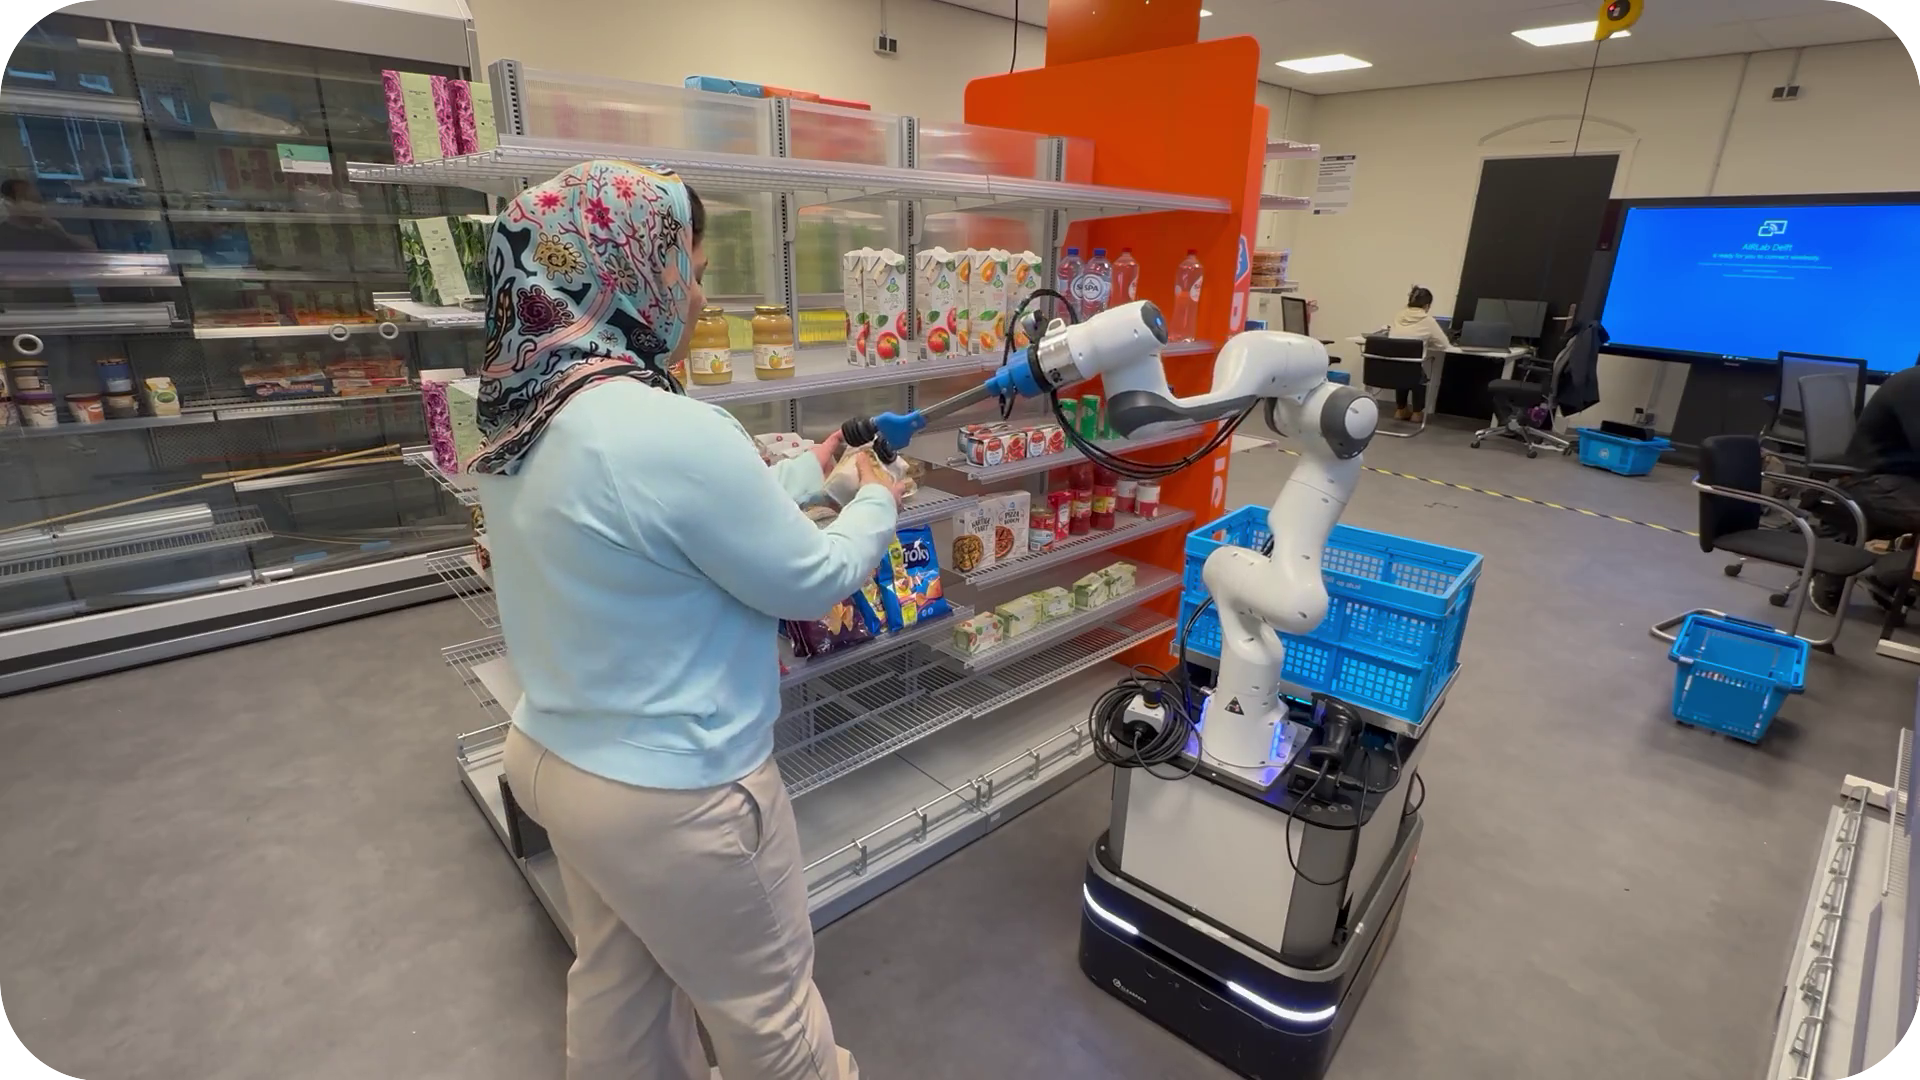
\includegraphics[width=0.9\textwidth]{src/introduction/img/collaborative_robot.png}
    \caption{Collaborative robot}
    \label{fig:collaborative_robot}
  \end{subfigure}
  \caption[]{The difference between environments where robots
  used to live in (left) \footnotemark and where we expect them to operate
  in the future (right).}
  \label{fig:different_robots}
\end{figure}

%  Mobility
Next to
safety, robots must be equipped with a similar level of
mobility as humans to perform meaningful tasks. Mobility of
industrial robots is limited as they are statically
attached to structural elements.
Placing
robots in environments, that are built with the mobility of
humans in mind, requires unlocking robots from their static
sockets.

In summary, to help aging societies in dealing with labor
shortage, the next generation of robots should be safe for
humans while equipped with the same level of mobility.

\subsection*{Mobile manipulation}
\label{sub:mobile_manipulation}

One key feature of modern robots, for human-shared
environments, is mobility. The combination of highly mobile
ground vehicles and manipulators is referred to as mobile
manipulation. This concept enables robots to navigate
\textit{and}
interact with their surroundings in ways previously deemed
challenging. By endowing robots with the ability to move and
manipulate objects in diverse environments, we further open
avenues for addressing the mentioned societal challenges.
Specifically, mobile manipulators could be used for tasks
from warehouse operations, restocking shelves, and package
delivery to intricate processes like food harvesting and
service tasks at home.
In short, mobile manipulation is a key concept if robots
should perform similar tasks as humans in the same
environments.

\footnotetext{
  Image from \url{https://www.vanch.net}.
}

\subsection*{Challenges in human-shared environments}
\label{sub:challenges_in_human_shared_environments}
%
However, despite their potential, robots are noticeably
absent from human-shared environments. The complexity of
such spaces, coupled with safety constraints, presents
formidable challenges. This is where \acf{tg}
becomes pivotal as one of the basic building blocks for
robotics software stacks. It determines the commands sent to
the motors in real-time, orchestrating a harmonious movement
that brings the robot closer to its goal while ensuring the
safety of itself and its environment.

While the hardware is ready for deployment, the
missing link lies in methods for generating trajectories
that prioritize safety while providing high success rates
and short cycle times.
This dissertation embarks on a journey to unravel this
critical aspect of robotics, exploring innovative \ac{tg}
methods that not only unlock the potential of
robotic hardware but also lead to a world where robots
seamlessly coexist with humans in shared spaces.
Importantly, the presented methods are all designed with
mobile manipulation in mind, as the increased level of
complexity of such systems may rule out some methods that
are superior for either the mobile base or the manipulator.

\section{Limitations of current approaches}
\label{sec:limitations_of_current_approaches}

In the quest for effective \ac{tg}, various
methods have been proposed, each with its set of advantages and
drawbacks.
The classical setup for robots --where they have
proven to be quite effective-- is behind fences. This setup
simplifies \ac{tg} dramatically as collision
avoidance can be done during the installation process and
trajectories can remain unchanged for the entire lifetime of
the robots. Therefore, high computational costs for
\ac{tg} are negligible as it is only performed
once during installation. However, their Achilles' heel lies
in their incapacity to adapt to dynamic, changing
environments.

Recognizing this limitation has led to the rise of local
\ac{tg} methods, especially as robots are
expected to enter human-shared environments. However, even
within this domain, challenges persist. Pure control
approaches, exemplified by operational space control or
impedance control, offer speed and interpretability but fall
short in incorporating the entirety of the problem, such as
collision avoidance with itself and the environment or
joint limit avoidance.


\subsection*{Optimization-based approaches}
With the aim of safe robots, many approaches are
rooted on optimization problems, centered around an
objective function and constraints that favor safety
guarantees and optimality. Such approaches are often
referred to as \acf{mpc} schemes or receding
horizon optimization \cite{hewing2020learning}. While
optimization-based methods have demonstrated success in
autonomous driving applications, they stumble when
confronted with real-time constraints in systems with
a large number of degrees of freedom due to high computational costs
\cite{spahn2021coupled}.

In the age of deep neural networks, learning-based
approaches have gained popularity as they promise similar
performance to optimization-based techniques. After all,
they solve the same problem, while changing the naming of
the objective function from cost function to loss (or
reward) function. Their major drawback lies in their
inability to integrate safety constraints in a principled
manner, and they are often prone to overfitting specific use cases during
training and thus lacking generalizability when confronted
with new scenarios \cite{noroozi2023conventional}.
Computational costs are also often
mentioned when criticizing such approaches, but as
computational capacity increases rapidly and important
advancements in natural language processing resulted from
more capable hardware and larger datasets
\cite{radford2023robust},
it seems little
justified. 

\subsection*{Control-based approaches}
In the early days of robotics, potential field methods were
popular in the context of \ac{tg}.
They are based on the idea of modeling the robot as
a point in a potential field built in the robot's configuration
space, where the goal is a minimum
and obstacles are maxima
~\cite{barraquand1992numerical,hwang1992potential}. This
approach is known to be computationally affordable but
only covers the static components of the problem, and thus
does not naturally integrate the dynamics of the robot.

Another notable contender from the same era is Cartesian
impedance control, praised for its rapid responsiveness and
perceived safety, \cite{hogan1985impedance}. Cartesian
impedance control models the point of interest on the
kinematic chain, usually the end-effector, as a
spring-damper-system attracted to the goal pose. In contrast
to potential field theory, the motion of the robot is thus
taken intro consideration. However, it falls short by not
encompassing crucial components for collision-free
\ac{tg}, such as self-collision avoidance or joint-limit
avoidance.
Modeling the point of interest of the robot as a
second-order differential equation raises whether all
components of the \ac{tg} problem can be handled in this
way. 

We can observe that modern approaches to \ac{tg} focus on
the practical side of \ac{tg} and often ignore the
underlying geometric structure \cite{Ratliff2015}. For
example, formulating the \ac{tg} problem in the Euclidean
work space of the end effector, as it is done in many
optimization-based methods and learning approaches, is a
simplification of the problem that ignores the configuration
space of the robot. Effectively, this approach uses a
Euclidean geometry. In contrast, the work space can also be
modeled as a Riemannian (or even non-Riemannian) manifold of
the configuration space \cite{klein2023design}. Then, other
components, that live in different manifolds of the
configuration space, can be seamlessly integrated into the
\ac{tg} problem \cite{Ratliff2015}. This insight has led to
a series of works where \ac{tg} has been addressed
purely geometrically
\cite{Ratliff2015,Ratliff2018,Cheng2020,Cheng2020a,Ratliff2020,Xie2020}.

\section{Geometries in trajectory generation}
\label{sec:geometries_in_trajectory_generation}

In this dissertation, we recall and extend a framework
that allows to iteratively design \ac{tg} via
summation of individual behaviors. Individual behaviors are
designed as differential equations of second order for which
stability properties are conserved during summation.
This concept, elegantly formalized as \ac{fabrics}, offers
a nuanced understanding of \ac{tg}.
Informally speaking, the composition shapes the
landscape on which the trajectory is then generated.
Formally speaking, we gradually introduce terms into the
non-Riemannian metric, shaping a smooth manifold of the
configuration space.

\section{Contributions}
\label{sec:contributions}

There are two lines of research in this thesis. Given the
success of \ac{mpc} in the field of autonomous driving and
mobile robotics, we explore how this method can be adapted
to mobile manipulation. 
%
\begin{textbox}{Part1Color}{Part 1: \acl{mpc}}
  As manipulators and even more so mobile manipulators are
  characterized by a high number of degrees of freedom, this
  thesis investigates how \ac{mpc} formulations known from
  autonomous driving must be adapted and how
  it performs in comparison to geometric methods.
\end{textbox}
%

As the results from the first part reveal that \ac{mpc} is 
not competitive in terms of reactivity and computational
costs, the second, and main part, of this thesis focuses on
geometric methods. Specifically, we study the framework
of \acl{fabrics} and its suitability for mobile manipulation
in dynamic environments.
%
\begin{textbox}{Part2Color}{Part 2: \acl{fabrics}}
  The main part of this thesis is dedicated to the
  exploration of the geometric framework of \ac{fabrics} for
  mobile manipulation in dynamic environments. In that
  context, we investigate how the framework generalizes to
  dynamic environments, how global path planning can be
  integrated and how implicit environment representations,
  such as point clouds can be used for collision avoidance.
\end{textbox}

To address the challenges formulated above, several
contributions are made in this thesis.

\paragraph{Mobile manipulation through \ac{mpc}}
\cref{cha:icra_21} presents an \ac{mpc} formulation for
whole body mobile manipulation. The presented method proposes to cope
with poor scaling in the number of collision constraints, by
using the concept of \acf{fsd}. This method achieves a
control frequency of 10Hz \textit{independent} on the amount
of collision obstacles in the environment.

\paragraph{Generalization of \ac{fabrics} to \ac{df}}
\cref{cha:tro_23} generalizes the framework of \ac{fabrics}
for dynamic environments. We refer to the resulting
framework as \ac{df}. Specifically, we introduce
time\hyp{}parameterized manifolds to integrate moving
obstacles and time\hyp{}parameterized goal definitions.
Technically,
we prove that energy conservation is preserved when
\textit{pulling} time\hyp{}parameterized components into
the configuration manifold. 
Similarly, we prove convergence to
time\hyp{}parameterized goals under a simple construction
condition. Quantitative comparisons between our method
and the original framework of \ac{fabrics} reveal
that failures due to collision is reduced from 9/20
to 0/20 for a 7-\ac{dof} robot in a real-world experiment.
In terms of path following, trajectories generated
with \ac{df} achieve a by a factor of 2 reduced summed error 
when compared with the original framework of
\ac{fabrics} for a 7-\ac{dof} robot in simulation.


\paragraph{Symbolic implementation of \ac{fabrics}}
As \ac{fabrics} offer a closed-form solution to
\ac{tg}, we present a symbolic implementation of
\ac{fabrics} in \cref{cha:icra_23}. This reduces
solver times to approximately 1ms for a 7-\ac{dof} robots, 
because the fabric composition, combining
the individual behaviors, is pre-computed and not
performed at runtime. The \ac{tg} policy can be
arbitrarily parameterized, and is thus suitable for
parameter refinement at runtime.
\cref{cha:icra_23} proposes the use of Bayesian optimization for
automated parameter tuning of \ac{fabrics},
reducing the need for expert knowledge. We show that
expert level tuning can be achieved without prior
knowledge of the framework. Additionally, tuning can
be transferred to different robots without substantial
loss of performance.

\paragraph{Implicit environment representations}
\cref{cha:ral_24} integrates implicit environment
representations into the framework of \ac{fabrics}.
This allows for the relaxation of the requirement for
the perception pipeline, as the environment is
represented implicitly in the policy.
Specifically, we compare \ac{fsd}, \ac{sdf} and raw
point clouds as the input for collision avoidance.

\paragraph{Demonstration in a Real-world setting}
\cref{cha:rss_24} demonstrates the usability of \ac{fabrics}
in a prototype application, specifically in the
context of order-picking in supermarkets, showcasing
real-world applicability and effectiveness. In this
real-world scenario, we make use of the ability
to arbitrarily formulate goals in different task
spaces. The goal definition of pointing towards the
shelf can then be very different to the goal
definition of placing an item in the shopping basket.

These contributions collectively advance the field of
\ac{tg} for mobile manipulation, offering novel
solutions to address key challenges and paving the way for
future research and development efforts.

\section{Outline}

The outline of this thesis is depicted in \cref{fig:outline}.
%
\begin{figure}[ht]
  \begin{center}
    \input{src/introduction/img/visual_outline.pdf_tex}
  \end{center}
  \caption{Outline of this thesis. General chapters are
  colored in blue, chapters related to \ac{mpc} are colored
  in red, chapters related to \ac{fabrics} are colored in 
  green, and demonstrations are colored in yellow.}
  \label{fig:outline}
\end{figure}
% state
After this introduction, \cref{cha:state} first introduces
relevant literature in the field of \ac{tg}
and motion planning.
% background
Then, \cref{cha:background} summarize the required tools
from optimal control and from differential geometry to
understand used in this thesis.
% mpc
\cref{cha:icra_21} explores an \ac{mpc}
formulation for whole body control
with a mobile manipulator. Specifically, we integrate
\acl{fsd} to cope with poor scaling in the number of
obstacles.
% dynamic fabrics
In \cref{cha:tro_23}, we derive a
generalization of optimization fabrics to dynamic
environments, including path following and avoidance with
moving obstacles.
% symbolic implementation
\cref{cha:icra_23} highlights the benefits of
formulating \ac{tg} in a symbolic way to
improve real-time capabilities and allow for online
parameter tuning.
% environment representations
\cref{cha:ral_24} showcases the integration of
implicit environment representations into the framework of
\ac{fabrics} to relax the requirements for the
perception pipeline.
% demo paper
\cref{cha:rss_24} showcases the 
usage of \ac{fabrics} in a prototype application in the
context of order-picking in supermarkets.
% conclusion
Finally,
\cref{cha:conclusion} summarizes the findings, their potential impact
on deploying robots in human-shared environments, discusses
the main differences between the presented methods and gives some
recommendations for future direction of research.


